\subsection{Experiments and Results}
%----------------------------------------------------------------------------------------------------------------------------------------------------------------------------------------------------------------------------------

In the experiments, we first evaluated the time to create each test suite in comparison between \evo and \codepro. As shown in Figure ~\ref{fig:Time}, \codepro generated test suites much more quickly than \evo did. Although \evo consistently takes longer to generate tests regardless of number lines of code and the complexity of the test suite. However, when comparing the complexity of the source code to the time to generate and the complexity of the test suites themselves, there is a clear trade off between time and complexity.

\begin{figure*}[!t]
\centering
  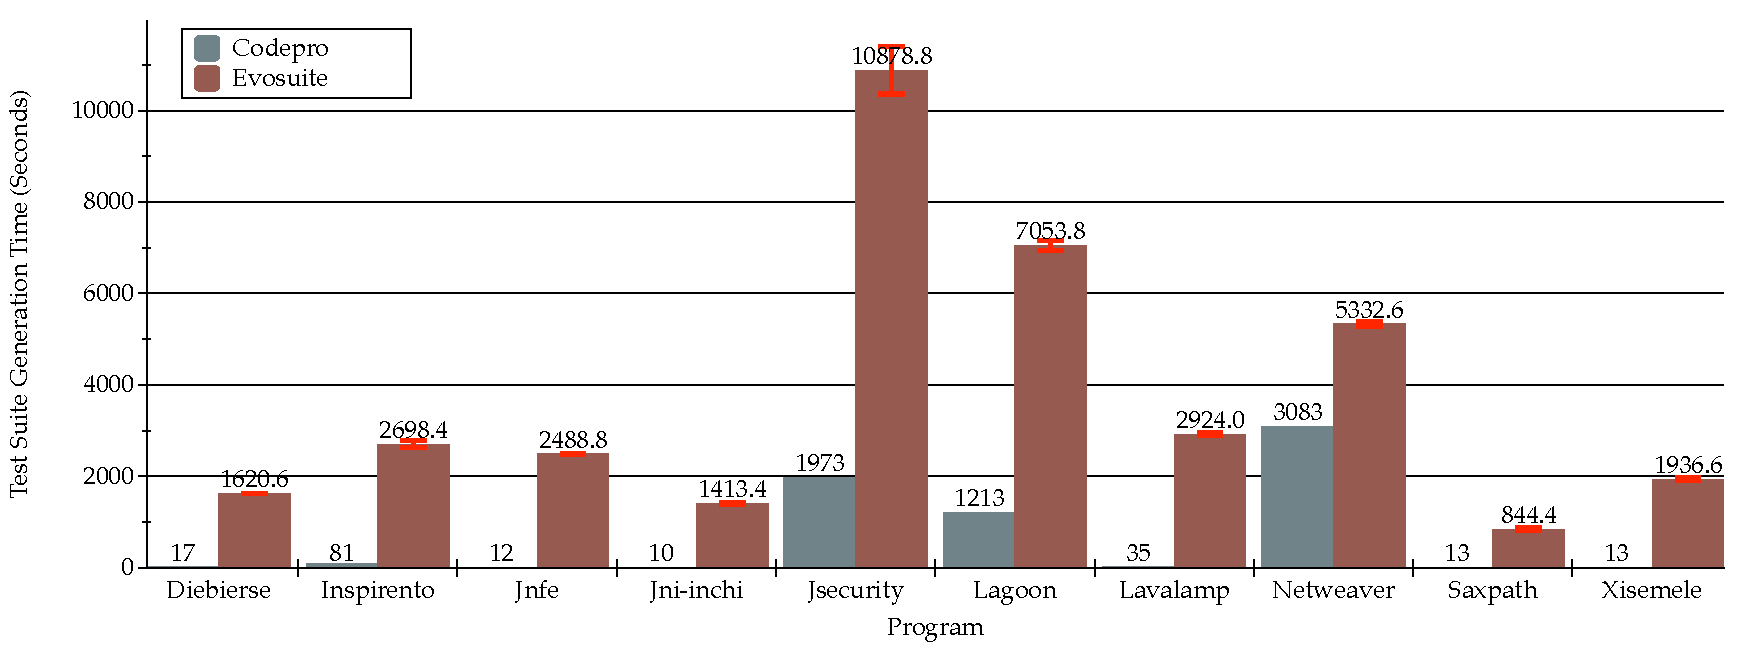
\includegraphics[width=\linewidth]{Time}
    \caption{Time to Generate Test Suite}
  \label{fig:Time}
\end{figure*}

\begin{figure*}[!t]
\centering
  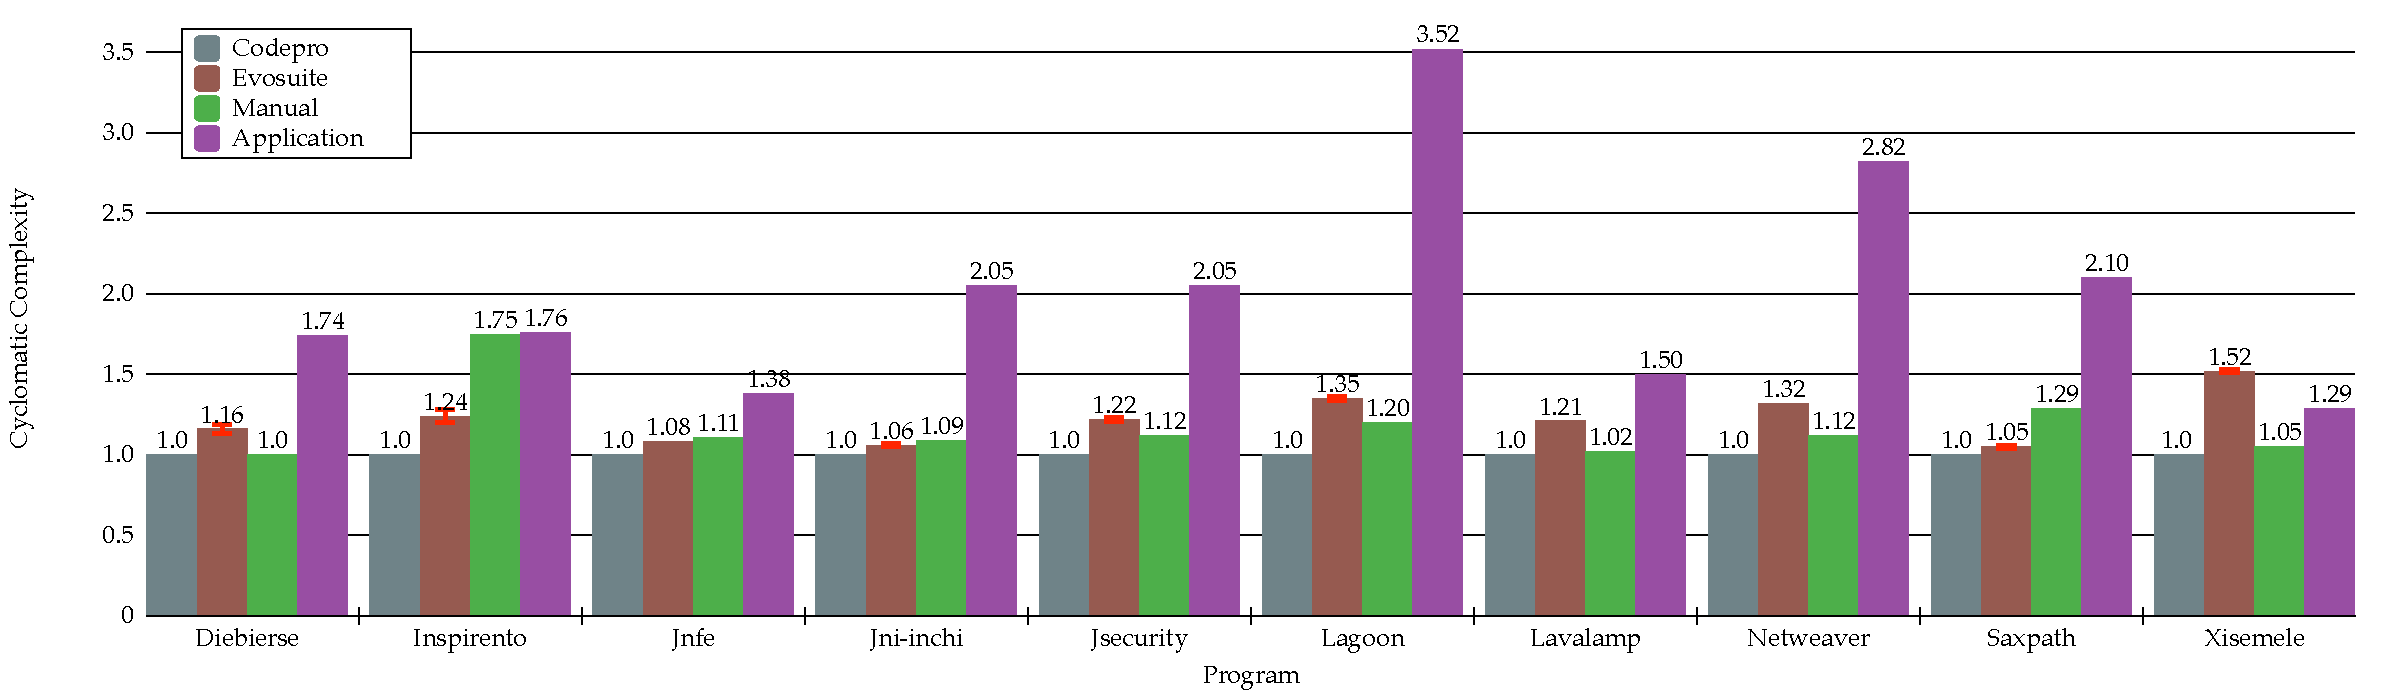
\includegraphics[width=\linewidth]{Complexity}
   \caption{Cyclomatic Complexity of Test Suites and Source Code}
  \label{fig:Complexity}
\end{figure*}

In Figure~\ref{fig:Complexity}, we list the complexities of the source code of the program, and the generated test suites from manual, \evo, and \codepro. Note that more complex tests can be more difficult to maintain. The \evo test suites are generally more complex than the other two, whereas \codepro is consistently at a lower complexity level. Due to increased complexity of the test suites, it can take more time create and run them~\cite{alspaugh:2007}. As evidenced by Figure~\ref{fig:Time_Complexity}, this indeed seems to be the case. In this data set, it would seem that the more complex the source code is, the more complex the tests are. Furthermore, the more complex the tests are, the longer the test generation takes to complete. This Figure displays the complexity of the test suite versus the time it took to generate the test suite. 

\begin{figure*}[!t]
\centering
  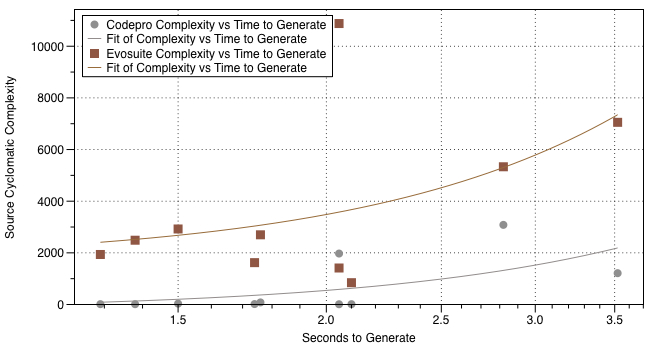
\includegraphics[width=\textwidth]{Time_Complexity}
    \caption{Time to Generate vs. Test Suite Cyclomatic Complexity}
  \label{fig:Time_Complexity}
\end{figure*}


\codepro maintains a low complexity level, but in doing so, this may lead to an inability to address complex code that requires deeper test cases. Although there is a performance boost in the speed to generate the test cases, one must also further examine the quality of the tests that are generated. \evo is more complex than the manually generated tests, which may mean that \evo cover deeper cases. If the depth of the tests are deeper in \evo, than one would expect the mutation scores to increase because the quality of tests would be higher. 

Using mutation scores as a measurement for quality of the tests, we then observe the overall mutation scores given to manual, \evo, and \codepro test suites in Figure~\ref{fig:Mutation_Score}. Manual tests generate higher mutation scores in four of the programs, whereas \evo also receives higher mutations scores for half of the programs. \codepro receives the highest mutation score for one of the programs by a small margin, but for the rest of the test suites, the scores are the lowest by a large gap. Only in \diebierse did \evo vary greatly in the scores received. This indicates that although the average mutation score for \evo is within a more unpredictable range of results in one case, on average \evo can match the mutation score and quality of the manually written tests.

\begin{figure*}[!t]
\centering
  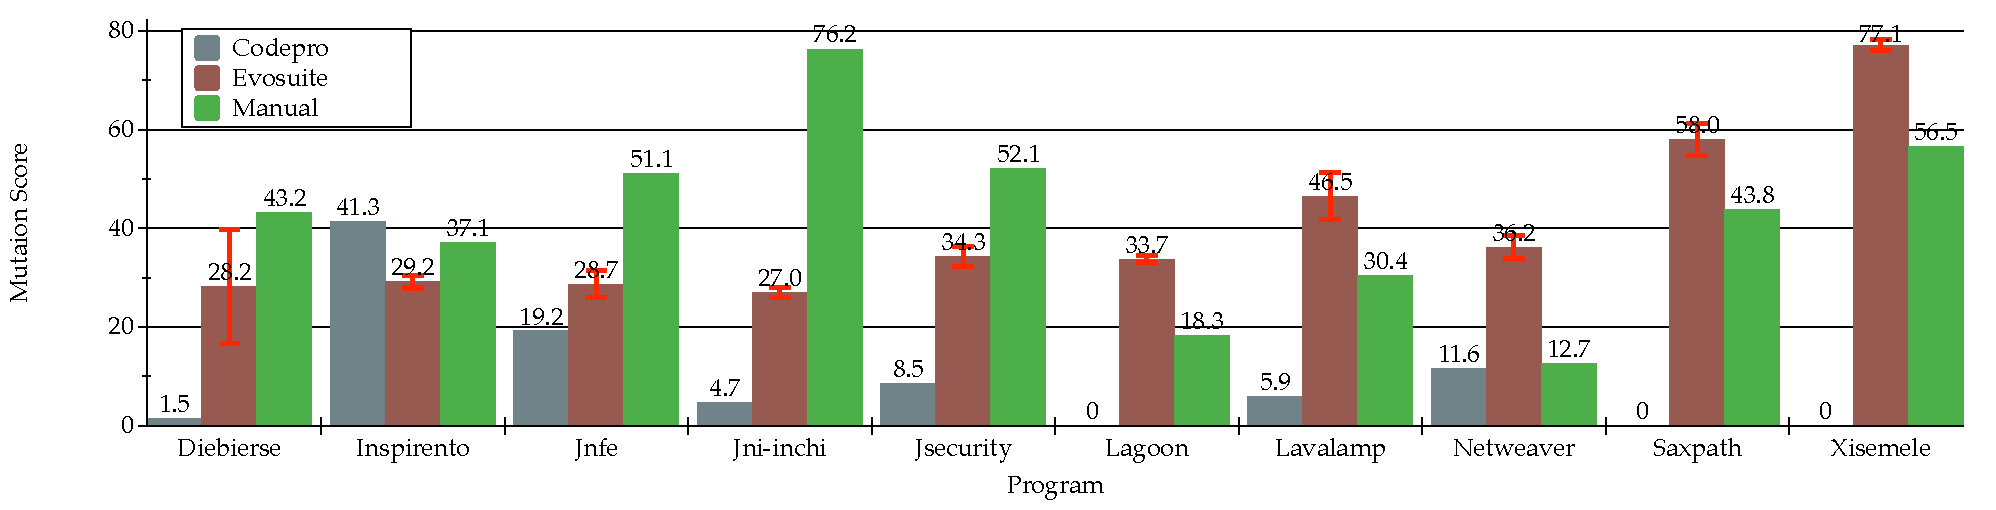
\includegraphics[width=\textwidth]{Mutation_Score}
    \caption{Mutation Score}
  \label{fig:Mutation_Score}
\end{figure*}

To further examine the cause of this, Figure~\ref{fig:Complexity_Mutation}describes the relationships between the mutation score of the test suites and the complexities of the source code. Notice that the manually written tests retain the highest mutation score overall at first. As the complexity of the program increases over time, the mutation score begins to drop. Around a cyclomatic complexity of 2.3, we find that \evo's retains a higher mutation score than manually written tests. \codepro overall receives abysmal mutation scores, and as the cyclomatic complexity of the program increases, the mutation score drops to 0.

This graph is an eye opener to the reality of capturing deeper test cases. Up until a certain point human beings can write deeper test cases to more complex functions. Once the programs become complex, it may be too difficult for a person to cover complex parts of code that require deeper test cases. \evo may be at an advantage with its learning algorithm that modifies itself over time to improve the mutation score. With \evo seeming to edge out the other two methods in terms of depth, one must also examine the breadth each of the tools can cover as well.

\begin{figure*}[!t]
\centering
  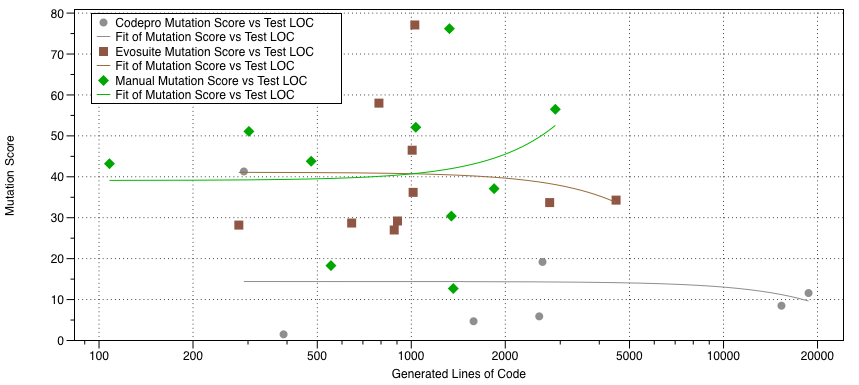
\includegraphics[width=\textwidth]{LOC_Mutation}
    \caption{LOC vs. Mutation Score}
  \label{fig:LOC_Mutation}
\end{figure*}


In Figure~\ref{fig:LOC_Mutation} the relationship between lines of code of the test suite and mutation score gives an initial impression that automated test suites lack the efficiency of a manually written test suite. \codepro not only results in the lowest mutation scores, but also creates the largest test suites. In the research, we found many of the test cases generated by \codepro were empty and contained comments for developers to put tests into templates. This reveals a different function that \codepro, unlike \evo, may be able to provide to developers. 

Although at first glance one may assume that \codepro lacks any usefulness because the quality of tests are low, one could also say that the templates provided by \codepro may give developers the flexibility of modifying and improving the test suite. \evo tests are much more complex, and could be conceivably difficult to maintain if the developers wished to evolve the test suite on their own. The trade off between automated and manually written tests could be an argument of modifiability in this case. Although \evo scores close to manually written tests when it comes to quality, how would one go about improving the test suites to meet that level depth that manual tests cover in larger programs? The tests would need to be modifiable from a human perspective, which in this case, could be an issue with tests suites like \evo.

\begin{figure*}[!t]
\centering
  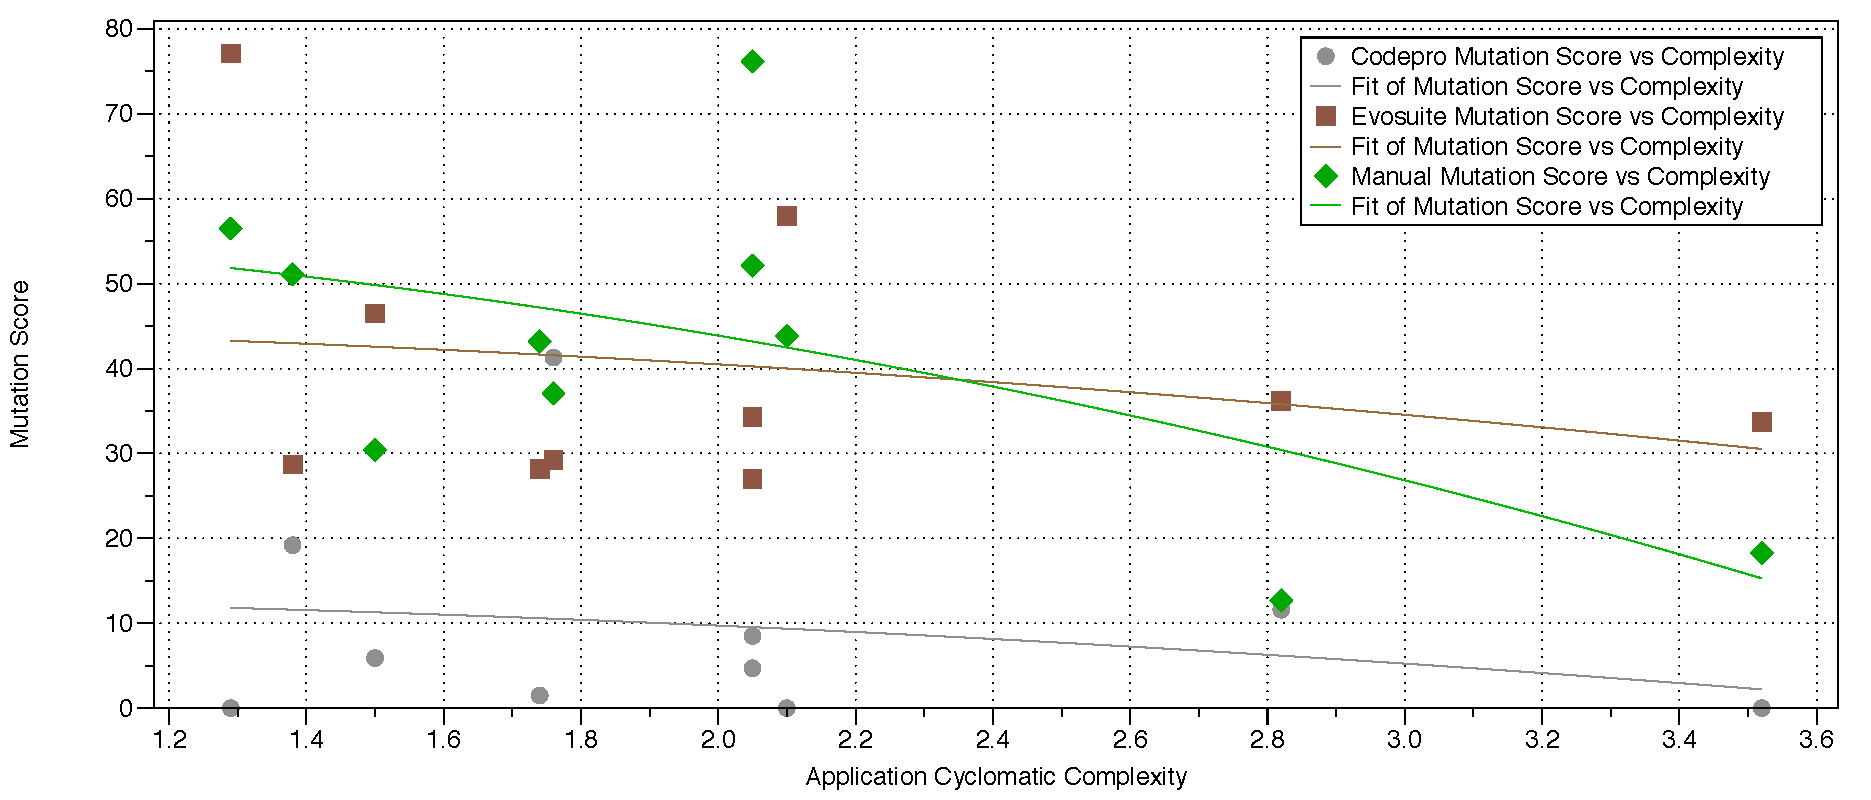
\includegraphics[width=\textwidth]{Complexity_Mutation}
    \caption{Mutation Score vs. Complexity}
  \label{fig:Complexity_Mutation}
\end{figure*}


Depth is important when evaluating the quality of tests, but breadth is an area one must consider when quantifying quality as well, as a test suite that deeply covers just one function will result in little breadth. In Figure~\ref{fig:Coverage},there is an extreme diversity of branch coverage amongst the three evaluated test suites. Overall, \codepro actually scores higher in branch coverage for four of the programs that were tested. \evo and the manually generated tests are tied for three programs in scoring the highest branch coverage. For the automated test generators, the branch coverages are closer on average, but manually written test suite scores seem to vary greatly. Again, this is probably due to the inconsistencies in different developers writing their test suites. For example, the developers on \lavalamp could have focused on a TDD philosophy in development, which would predictably yield higher test coverage. However, the developers for \netweaver may have only been concerned with testing one part of their code, and thus branch coverage remained low. In fact, unit tests for only complex parts of the code are common in development, and thus this chart alone only reveals the inconsistent nature of how developers write unit tests. One must look further at the mutation the branch coverage to reach a more definitive 

\begin{figure*}[!t]
\centering
  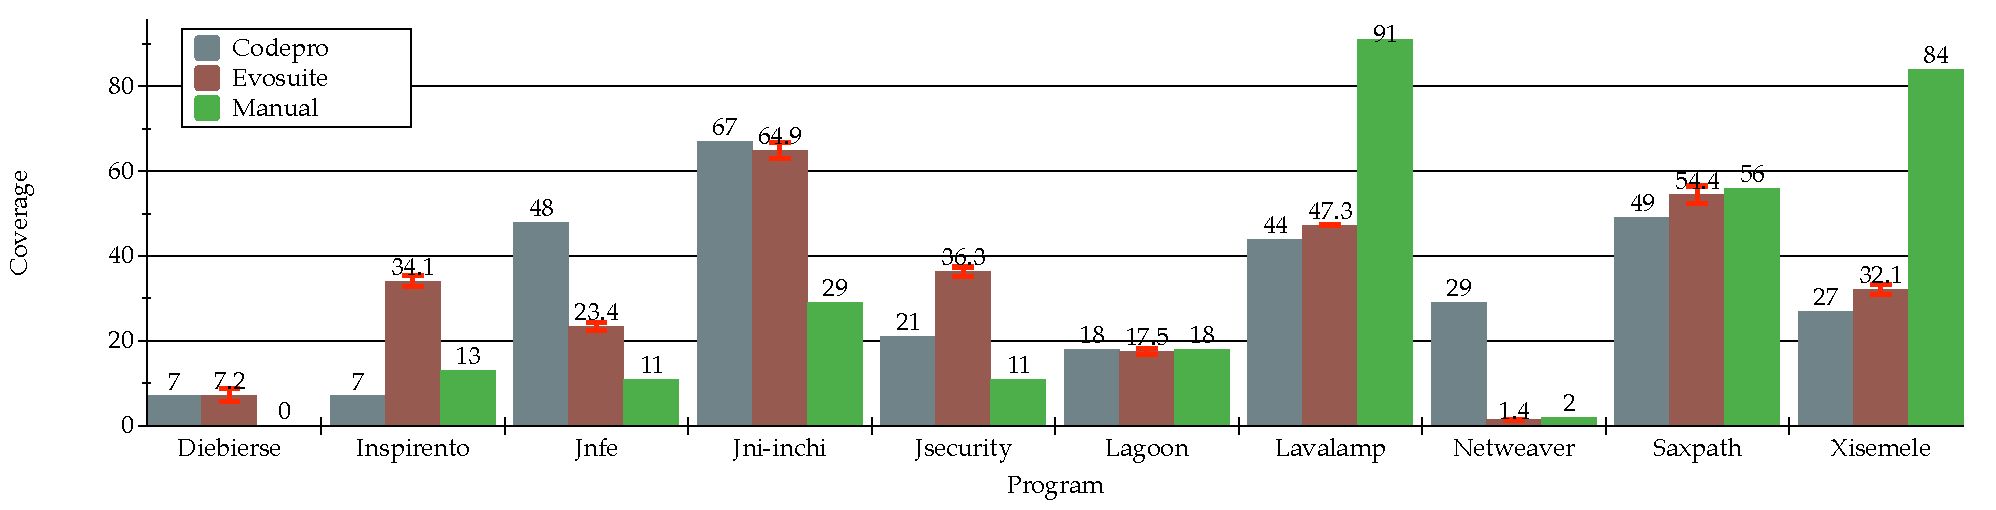
\includegraphics[width=\textwidth]{Coverage}
    \caption{Coverage}
  \label{fig:Coverage}
\end{figure*}

Finally, we examined the center piece of the results, in comparing the evaluation of mutation scores and branch coverage. In Figure~\ref{fig:Coverage_Mutation}, we compare the mutation score (depth) to the branch coverage (breadth) of the test suites. \codepro falls short in the mutation scores, but does have higher branch coverage coverage scores. As the branch coverage increases however, the mutation score in \codepro dips drastically. Understanding that the mutation score was never good to begin with in \codepro, this leads us back to the discussion in perhaps using \codepro as template tool rather than a upfront ready-to-go test suite. Although the mutation scores are low, the coverage is high, providing a large amount of tests for developers to look at and fill over time. 

More interesting are the similar trends between manual and \evo generated test suites. Initially \evo begins a bit lower in mutation score and branch coverage, but as the branch coverage increases, it would seem that \evo surpasses the Manual tests in quality. Overall, the quality of manual tests seems to rise above \evo ever so slightly. However, the trends seems to indicate that \evo will generate tests that will cover more code with better quality than manually written test suites, although both systems increase in quality as the test branch increases.

\begin{figure*}[!t]
\centering
  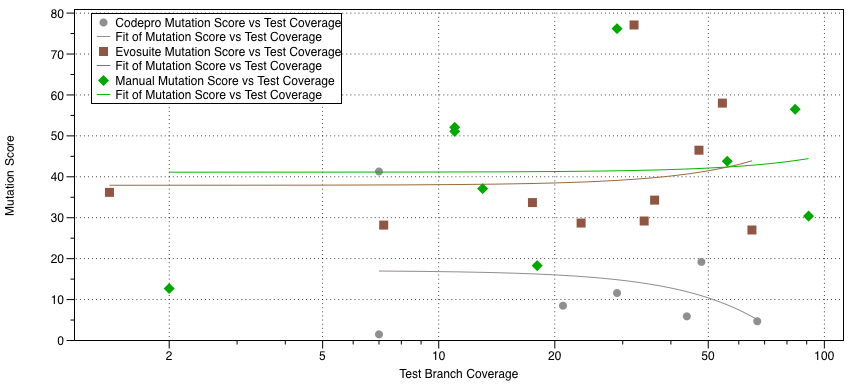
\includegraphics[width=\textwidth]{Coverage_Mutation}
    \caption{Coverage vs. Mutation}
  \label{fig:Coverage_Mutation}
\end{figure*}
